\documentclass{article}
\usepackage{polyglossia}
\usepackage[a4paper]{geometry}
\usepackage{mathtools, amssymb, amsfonts}
\usepackage{amsthm}
\usepackage{fontspec}
\usepackage{titling}
\usepackage{float}
\usepackage{listings}
\usepackage{graphicx}
\usepackage[hidelinks]{hyperref}
\usepackage{tikz}
\usepackage[locale = FR, exponent-product = \cdot, inter-unit-product = .]{siunitx}
\usetikzlibrary{shapes,calc}
\usepackage[shortlabels]{enumitem}
\usepackage{comment}

\setdefaultlanguage{french}


%% Math commands
\renewcommand{\vec}[1]{\mathbf{#1}}
\renewcommand\epsilon\varepsilon
\renewcommand\phi\varphi
\newcommand{\N}{\mathbb N}
\newcommand{\Z}{\mathbb Z}
\newcommand{\R}{\mathbb R}
\newcommand{\Q}{\mathbb Q}
\newcommand{\CC}{\mathbb C}
\newcommand{\K}{\mathbb K}
\DeclarePairedDelimiter{\abs}{\lvert}{\rvert}
\DeclarePairedDelimiter{\norm}{\lVert}{\rVert}

%% Math environments
\theoremstyle{definition}
\newtheorem{exo}{Exercice}

\theoremstyle{remark}
\newtheorem*{rap}{Rappel}

%% Titling configuration
\pretitle{\begin{center}\LARGE\textsf }
\title{Électrostatique}
\posttitle{\par\end{center}\vspace{-1.2em}}

\preauthor{}
\author{}
\postauthor{}

\date{\today}

\begin{document}
\maketitle


\section{Notion de charge électrique}

\subsection{Généralités}

La \textit{charge} est, comme la masse, une grandeur permettant de décrire les propriétés physique de la matière. Ici, il s'agit des propriétés concernant son comportement lorsqu'elle est plongée dans un champ électromagnétique (un champ électrique seul, un champ magnétique seul, des ondes radios, la lumière...). Son unité est le \textit{coulomb} (C).

La charge est une caractéristique particulièrement pertinente pour les particules subatomiques, telles que les électrons, protons, muons... La plus petite charge possible pour la plupart de ces particules, appelée \textit{charge fondamentale}, est $e= \SI{1.6e-19}{\coulomb}.$

\vspace{1em}
\fbox{
\parbox[c]{0.94\textwidth}{
\textbf{\textsf{Note historique}} La charge électrique est découverte par les Grecs de l'Antiquité, qui remarquent que les petits boutons d'ambre ornant leurs habits, après avoir frotté avec ceux-ci, se mettent à attirer des petits objets tels que des cheveux. En frottant suffisamment, ils observent même la production d'une étincelle.
}}

\vspace{1em}

Les charges ont un signe: négatif ou positif. Les électrons portent une charge négative de $-e$, les protons une charge positive de $+e$. Dans l'exemple des boutons d'ambre des Grecs, ceux-ci portent une charge négative puisque le fait de les frotter arrache des électrons à la surface contre laquelle ils frottent.

Encore des exemples : lorsque vous enlevez votre pull ou que vous vous peignez ou brossez les cheveux, vous entendez un léger craquement, qui peut même s'accompagner, à luminosité faible, de la présence d'étincelles.

\subsection{Charge d'un système de particules}

Étant donné un système de $N$ particules portant des charges $q_1,\ldots,q_N$, la charge totale du système formé est 
\[Q = q_1+\cdots+q_N.\]

On dit que le système est \textit{électriquement neutre} si $Q=0$. Un système de particules portant chacune des charges électriques différentes peut donc être globalement électriquement neutre.

\paragraph{Quelques exemples.} \begin{itemize}
	\item Les molécules sont globalement neutres, alors qu'une molécule telle que l'eau peut porter des charges partielles, dues à la forte électronégativité de l'atome d'oxygène. 

\begin{figure}[H]	
	\centering
    \begin{tikzpicture}
    \tikzset{dot/.style={circle,fill,inner sep=2pt}};
	\node (H1) at (-0.65,-0.8) [dot,label={below left:H},label={above left:$+\delta e$}]{};
	\node (H2) at (0.65,-0.8) [dot,label={below right:H},label={above right:$+\delta e$}]{};
	\node (O) at (0,0) [dot,label={left:O},label={above right:$-2\delta e$}]{};	
	\draw (H1) -- (O) -- (H2);
	\end{tikzpicture}
	\caption{La molécule d'eau est globalement électriquement neutre, mais chaque atome porte une charge partielle.}
\end{figure}

\begin{rap}
	L'électronégativité est la tendance d'un élément à attirer vers lui et s'accaparer, en quelque sorte, les électrons mis en jeu lors d'une liaison covalente. Le rapport des électronégativités entre les éléments en jeu dans une liaison covalente détermine si l'un d'entre eux va remporter une charge partielle, et le cas échéant c'est l'élément le plus électronégatif. Selon l'échelle de \textsc{Pauling}, les éléments les plus électronégatifs sont ceux qui se trouvent vers le haut et vers la droite du tableau périodique des éléments (hormis les gaz nobles). Ainsi, l'oxygène n'est devancé que par le fluor ($\mathrm{F}$) en terme d'électronégativité.
\end{rap}

\item Le sel, cristal ionique de formule $\mathrm{NaCl}$, composé des ions chlorure $\mathrm{Cl}^{-}$ et sodium $\mathrm{Na}^+$, est globalement neutre, même si chaque ion composant chaque maille de ce cristal est électriquement chargé.

\begin{figure}[h]
	\centering
	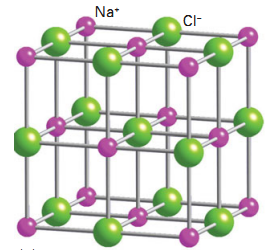
\includegraphics[width=0.36\textwidth]{parts/electrostat/sel_cristal.png}
	\caption{La structure cristalline du sel. Les ions chlorure et sodium sont arrangés dans un motif cubique}
\end{figure}

\begin{rap} Un cristal est un solide dont les constituants (atomiques, ioniques, moléculaires) sont arrangés dans une structure régulière, dans le sens où il existe un arrangement de base, un motif, appelé \textit{maille}, tel que le solide soit en fait un grand réseau où ce motif se répète à l'identique. D'autres exemples sont la neige, le sucre, la fibre de carbone.
\end{rap}

\end{itemize}

\section{Interaction électrostatique}

\subsection{Généralités}

Lorsque deux corps chargés électriquement sont mis en présence, comme un bouton d'ambre chargé et des cheveux, un peigne fraîchement sorti de ceux-ci et un filet d'eau, un pull et un ballon de baudruche, on observe les effets d'une force. En effet, ils se rapprochent (interaction \textit{attractive}) ou s'éloignent (interaction \textit{répulsive}).

Ce comportement est dû au fait que la présence de charges modifie les propriétés de l'espace en créant un \textit{champ électrique}, qui confère à chaque point de l'espace une direction privilégiée dans laquelle orienter les particules chargées et une intensité avec laquelle le faire. Ainsi, une charge qui se retrouve en présence d'une autre est happée par les effets du champ électrique crée par cette dernière.

Le \textit{champ électrique} est un champ vectoriel, c'est-à-dire une fonction d'une variable vectorielle (la position) à valeurs vectorielles (la direction et l'intensité du champ). On le note, classiquement, $\vec{E}$. La situation électrostatique correspond au cas où le champ électrique $\vec{E}$ est indépendant du temps.

L'électrostatique << classique >> (par opposition aux contextes de la théorie de la relativité d'\textsc{Einstein} ou la mécanique quantique de \textsc{Planck}, \textsc{Hilbert}, \textsc{Schrödinger}) est régi par les équations de \textsc{Maxwell} (1831-1879). 


\subsection{Champ électrique créé par une charge ponctuelle}

Pour le cas d'une charge ponctuelle $q$ située en l'origine, les équations de \textsc{Maxwell} conduisent à la solution
	\[ \vec{E}(\vec{r}) = \frac{1}{4\pi\epsilon_0}\frac{q}{\norm{\vec{r}}^3}\vec{r} \]
où $\epsilon_0\approx\SI{8.854e-12}{\farad\per\meter}$ est la permittivité électrique du vide (sa tendance à laisser passer les champs électriques). Le champ est donc \textit{radial} et ne dépend que de la distance $r=\norm{\vec{r}}$ : $\vec{E} = E(r)\vec{e}_r$, et pour $r=\mathrm{OM}$ on retrouve la formule familière
	\[
    E = \frac{1}{4\pi\epsilon_0}\frac{q}{\mathrm{OM}^2}.
    \]

\begin{figure}[h]
	\centering
    \begin{tikzpicture}
    \tikzset{dot/.style={circle,fill,inner sep=2pt}};
	\node (ch) at (0,0) [dot,label={$q$}]{};
    
	\end{tikzpicture}
    \caption{Champ électrique créé par une charge ponctuelle $q$ placé en l'origine $O$.}
\end{figure}

\begin{rap}
	On a $k=\dfrac{1}{4\pi\epsilon_0}=\SI{9.0e9}{\meter\per\farad}.$
\end{rap}








\end{document}